%% LyX 2.1.2 created this file.  For more info, see http://www.lyx.org/.
%% Do not edit unless you really know what you are doing.
\documentclass[english]{amsart}
\usepackage[T1]{fontenc}
\usepackage[utf8x]{inputenc}
\usepackage{geometry}
\geometry{verbose,tmargin=2cm,bmargin=2cm,lmargin=2cm,rmargin=2cm,headheight=2cm,headsep=2cm}
\setcounter{secnumdepth}{3}
\setcounter{tocdepth}{3}
\usepackage{float}
\usepackage{amsthm}
\usepackage{amsmath}
\usepackage{amssymb}
\usepackage{graphicx}

\makeatletter

%%%%%%%%%%%%%%%%%%%%%%%%%%%%%% LyX specific LaTeX commands.
%% Because html converters don't know tabularnewline
\providecommand{\tabularnewline}{\\}

%%%%%%%%%%%%%%%%%%%%%%%%%%%%%% Textclass specific LaTeX commands.
\numberwithin{equation}{section}
\numberwithin{figure}{section}

%%%%%%%%%%%%%%%%%%%%%%%%%%%%%% User specified LaTeX commands.
\usepackage{babel}

\makeatother

\usepackage{babel}
\begin{document}

\section*{Questions posées : }

Effet du nombre de villes k à population globale constante sur le
taux d'extinction ? A phase constante 0, pi/4, pi/2, 3pi/4 et pi 


\subsection*{a. tau décroit-il avec la synchronie (à N et k constant) ? Comment
en fonction de N et k ?}


\subsection*{b. tau croit-il avec k (N constant) ? Comment en fonction de la synchronie ? }


\subsection*{c. tau décroit-il avec N (k constant) ? Comment en fonction de Phi ?
CCS Critical Community Size}


\subsection*{d. Influence du taux de contact}


\subsection*{e. Influence du couplage }


\subsection*{f. Comment augmenter le taux d'extinction (i.e augmente la synchronie)
par une vaccination optimale ?}


\section*{Discussion : }
\begin{itemize}
\item Discussion sur Code EpiDynamics. 

\begin{itemize}
\item Giang a utilisé le package ode dans le cas déterministe. 
\item Sur les aspects stochastiques ; Pb de la comparaison des résultats. 
\item On peut utliser deux méthodes suivantes pour comparer les résultats :
\textbf{Kullback-Leibler Divergence Kolmogorov–Smirnov test }
\end{itemize}
\item Analyse des résultats Garder N constants et k sous-populations de
N/k, ajouter l'intervalle de confiance. 
\end{itemize}
\textbf{A faire : }
\begin{itemize}
\item Connaitre date de fin de troisième année : Partager le plan de thèse 
\item Donne le temps nécessaire pour répondre à chaque question. 
\item Enregistrer le nombre des extinctions locales et le nombre de recolonisation
locale.
\item ECRIRE : un rapport en latex/knitrR qui contient au moins les 3 sections : 
\end{itemize}
\pagebreak{}


\title{REMETTRE LES RESULTATS}

\maketitle
Here, we use the formula given by YANN. The fore of infection is proposed
for city $i$ :

\textbf{
\begin{equation}
\lambda_{i}=\sum_{j}\rho_{ij}\kappa_{j}\log\left[1-\sum_{k=1}^{M}\left(\frac{\left|I_{k,t}\right|}{N_{k}}\times c_{ik}\times\xi_{jk}\right)\right]\label{eq:force-1}
\end{equation}
 }where\textbf{ }$c_{i,k}$ ($0\leqslant c_{ij}\leqslant1$) is the
probability that a susceptible individual native from $i$ being in
contact with another infected individual native from $k$ gets infected.
$\xi_{jk}$ ($0\leqslant\xi_{ij}\leqslant1$) refers to the probability
that an individual $y$ meeting $x$ in $C_{j}$ comes from $C_{k}$.\textbf{
}$\kappa_{j}$ is the average number of contacts per unit of time
a susceptible will have when visiting city $j$. $\rho_{i,j}$ ($0\leqslant\rho_{ij}\leqslant1$)
is denoted as the probability that an individual from subpopulation
$i$ visits subpopulation $j$, of course, $\sum_{j=1}^{M}\rho_{ij}=1$.
We can verify that in the limit case on one single subpopulation in
the metapopulation ($i=j$ and $n=1$) we have 
\begin{equation}
\lambda_{i}=-\kappa_{i}\log(1-\frac{I_{i}}{N_{i}}\times c_{ii})
\end{equation}
 Consider that the average number of contacts per unit of time $\kappa_{i}$
is seasonally forced and seasonality is an annually periodic function
of time. As a result, for the subpopulation $i$ : 
\begin{equation}
\kappa_{i}(t)=\kappa_{i0}\left[1+\kappa_{i1}\cos\left(\frac{2\pi t}{T}+\varphi_{i}\right)\right]\label{eq:beta_i}
\end{equation}


In order to run simulations, we use the same values of all parameters
for all subpopulations. We have a table of the convenient values for
parameters of measles as follows :

\begin{table}[tbph]
\begin{centering}
\protect\caption{Some Disease Parameter Values for Measles from the Literature}

\par\end{centering}

\centering{}%
\begin{tabular}{lccc}
\textbf{parameter}  & \textbf{description}  & \textbf{value} & \textbf{unit}\tabularnewline
$\mu$  & birth and death rate per day  & $1/(70*365)$  & 1/(people{*}day)\tabularnewline
$\kappa_{0}$  & mean value of the number of contacts $\kappa$ per unit of time  & $\{30,50,80,100,150\}$ & people/day\tabularnewline
$\kappa_{1}$  & amplitude of the number of contacts $\kappa$ per unit of time  & $\{0.01,0.1\}$ & \tabularnewline
$\gamma$  & recovery rate per day  & $1/8$ & 1/(people{*}day)\tabularnewline
$\sigma$  & average exposed duration per day  & $1/5$ & 1/day\tabularnewline
$\rho$  & coupling rate & \textbf{$\{0,0.001,...,0.5,0.8,1\}$} & \tabularnewline
$\varphi_{max}$  & synchrony parameter in radian  & $\{0,\pi/4,\pi/2,3*\pi/4,\pi\}$ & radian\tabularnewline
$N$  & population size of subpopulation & $\{5e5,7e5,1e6,2e6,5e6\}$ & people\tabularnewline
$n$  & number of subpopulation & $\{2,3,...,10,15,20,30\}$ & subpopulation\tabularnewline
$t_{max}$  & simulation time & $100$ & day\tabularnewline
 &  &  & \tabularnewline
\end{tabular}
\end{table}



\section*{\textbackslash{}section\{Analysis of the variation of tau in function
of Phi\}}

\begin{figure}[H]
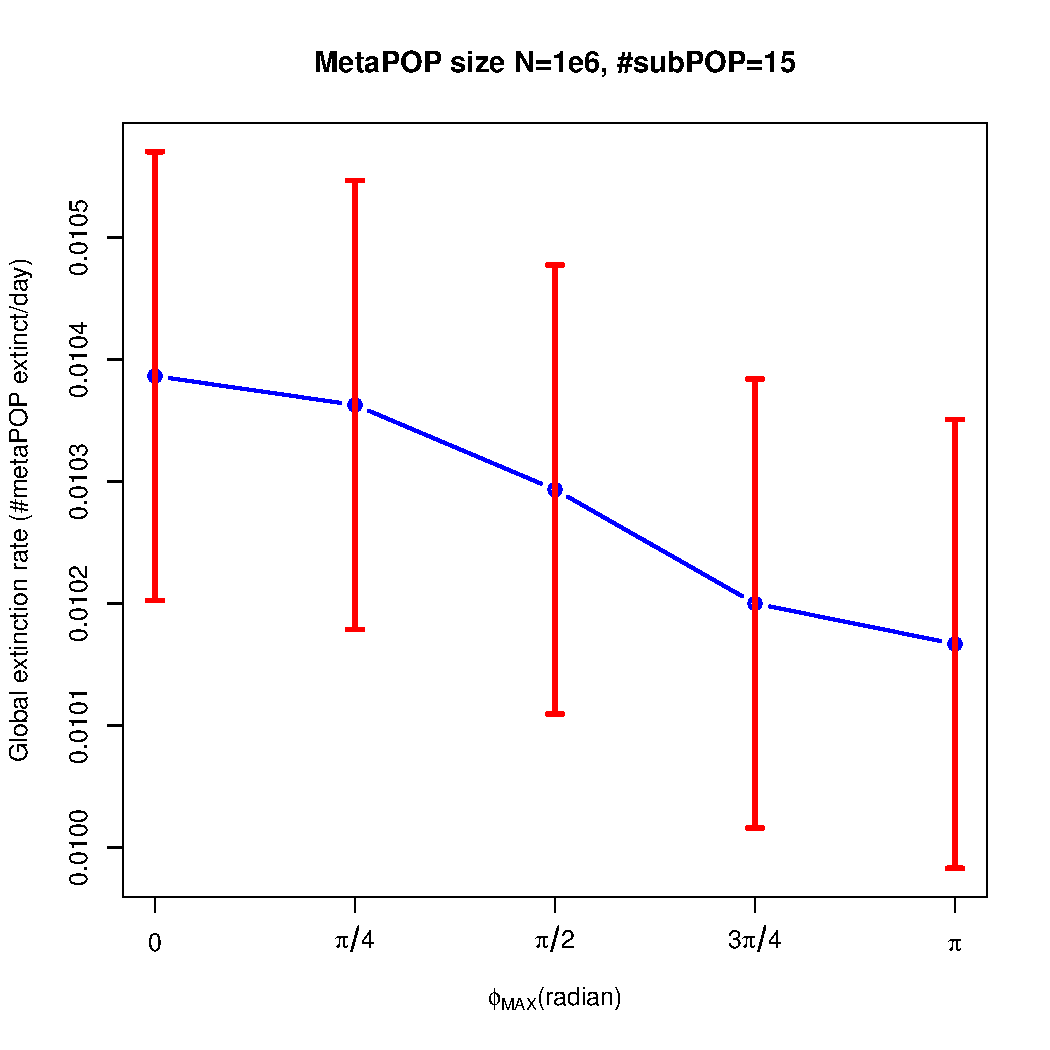
\includegraphics[scale=0.4]{plotIntvMeta15N1e6}

\protect\caption{Estimated global etinction rates in the metapopulation of fifteen
subpopulations after 100 different simulations with the metapopulation
size $N=10^{6}$, coupling rate $\rho=0.1$. Here, with 95\% confidence
interval, the red lines and the blue points are respectively the confidence
intervals and the estimated rates for the global extinction rate of
each value of $\varphi_{max}$.}


\label{FigNconstKconst}

\end{figure}

\begin{itemize}
\item Running time : 4.188hours
\item Analysis : The figure \ref{FigNconstKconst} shows to us that the
amplitude of the confidence intervals for each value of $\varphi_{max}$
are quite far to each other. Furthermore, it goes down robustly when
$\varphi_{max}$ runs from $0$ to $\pi$. The phase difference strongly
influences the global disease extinction rate. The figure \ref{FigNconstKconst}
indicates the trend of the extinction rate with decreasing the level
of asynchrony. The asynchrony between subpopulations is the main reason
why the infectious disease goes extinct in the slow way.
\end{itemize}

\section*{\textbackslash{}section\{Analysis of the variation of tau in function
of k\} }

\begin{figure}[H]
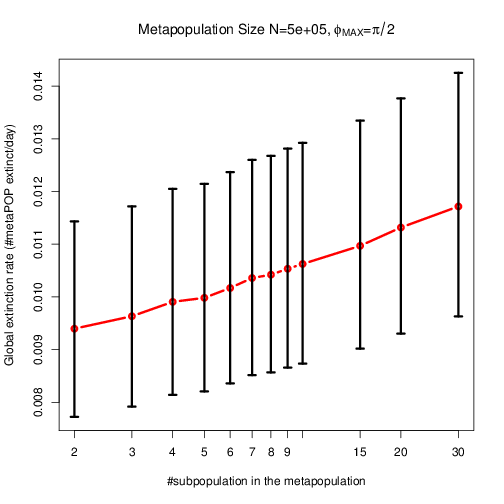
\includegraphics[scale=0.4]{plotTOTALnbvillesPhipi2}

\protect\caption{Estimated global etinction rates in different metapopulations after
100 different simulations with the metapopulation size fixed $N=5\times10^{5}$,
coupling rate $\rho=0.1$ and $\varphi_{max}=\pi/2$. Here, with 95\%
confidence interval, the black lines and the red points are respectively
the confidence intervals and the estimated rates for the global extinction
rate of each metapopulaion.}


\label{FigGlobExtNbVilles}
\end{figure}

\begin{itemize}
\item Running time : 8.589hours
\item Analyse : The result (figure\ref{FigGlobExtNbVilles}) exhibits to
us that the number of subpopulations strongly has an influence for
the disease persistence time. The global extinction rate of an infectious
disease in a metapopulation increases when the number of subpopulations
in this metapopulation increases. With the metapopulation size is
fixed, when the number of cities in the metapopulation goes up, it
means that the population size of each city is declined. In particular,
the population size of each city is very small when the number of
cities reaches to 30. The dynamic in a small population goes fastly
extinct. Althought, the model used is the coupling metapopulations,
there are interactions among subpopulations and recolonisations of
desease. But because the population size is small, the number of visiteurs
going to other city is very little. The time of disease persistence
in a population having the small size is short. We fastly find the
mass extinction in the metapopulation. In addition to the resultat
above, we have the relation between the local extinction number of
the metapopulation and its number of cities as follows (figure\ref{FigNbLocalExtNbVilles})
\end{itemize}
\begin{figure}[H]
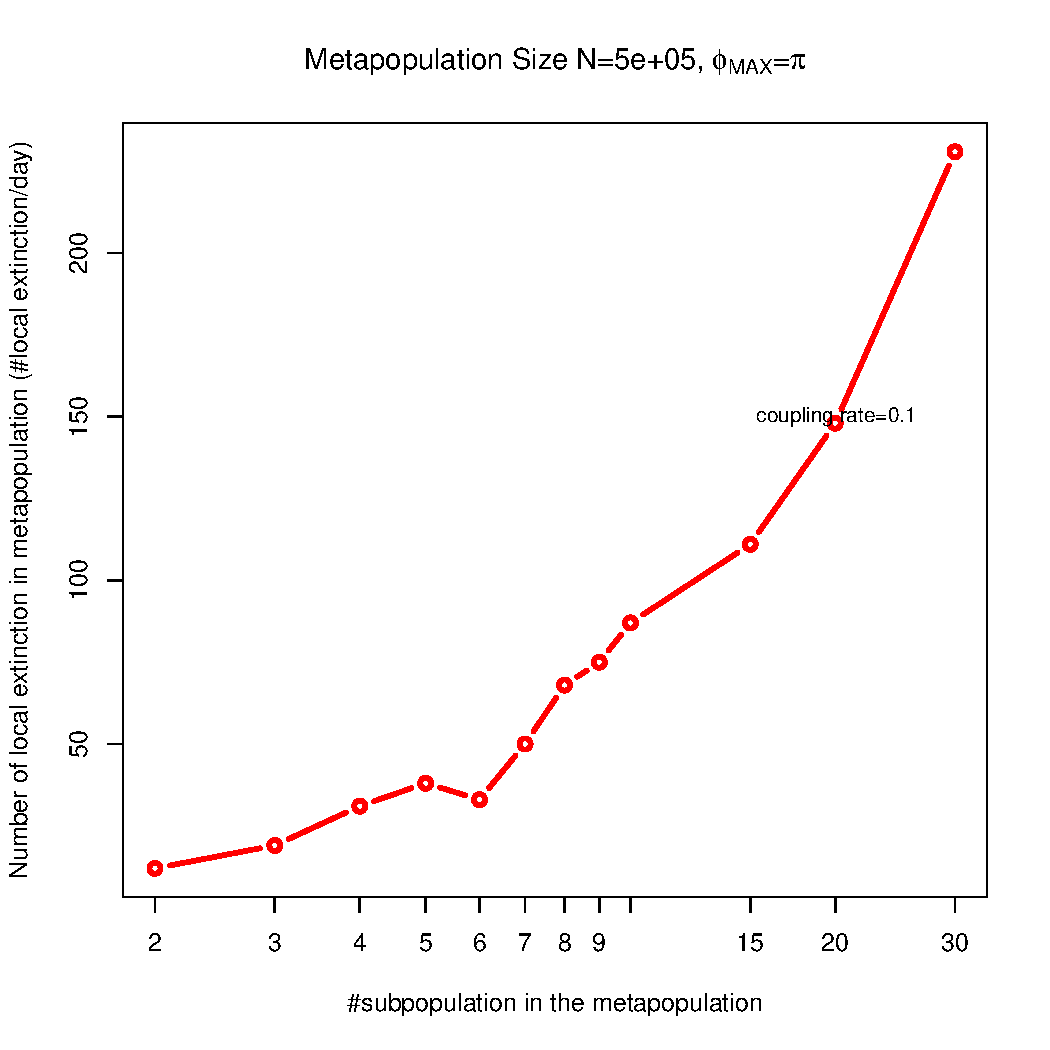
\includegraphics[scale=0.4]{plotTOTALnbvillesPhipi2_localEXT}

\protect\caption{Number of local extinction in the metapopulation with the size N=5e+05,
$\phi_{max}=\pi/2$}


\label{FigNbLocalExtNbVilles}
\end{figure}


As showed in the figure \ref{FigNbLocalExtNbVilles}, the number of
the local extinction in the metapopulation has an increase when the
number of subpopulation in the metapopulation rises from 2 to 30.
This is obvious that in the coupling metapopulation, there are the
interactions between cities. One city gets the local extinction but
it is fastly reinfected because of the migration of infected individuals
of the other cities.


\section*{\textbackslash{}section\{Analysis of the variation of tau in function
of N\}}

\begin{figure}[H]
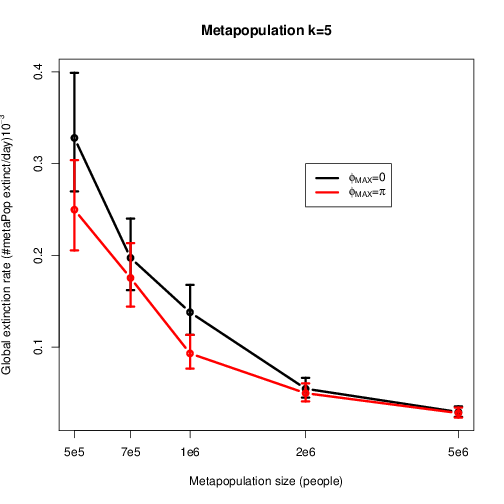
\includegraphics[scale=0.4]{resPOPSIZE_interval}

\protect\caption{The relation between the metapopulation size and the global extinction
rate for the metapopulation of five cities.}


\label{FigMetaSizeGlobExt}
\end{figure}

\begin{itemize}
\item Running time : 3 hours (3.231257hours)
\item Analysis : From the figure \ref{FigMetaSizeGlobExt}, we find that
the mass extinction rate goes down when the metapopulation size augments,
at the same time, these rates decreases when the asynchrony $\phi_{max}$
goes up. It is obvious that the metapopualtion size is big, then the
time of disease persistence augments, then the mass extinction rates
is declined.
\end{itemize}

\section*{\textbackslash{}section\{Influence du taux de contact\}}

\begin{figure}[H]
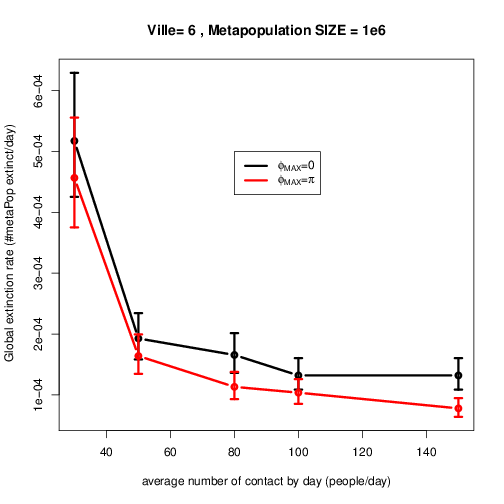
\includegraphics[scale=0.4]{plotresCONTACTvil6N1e6}

\protect\caption{Influence of the average number of contact per day }
\end{figure}

\begin{itemize}
\item Running time : 3.369hours
\item Analyse : Here we find that the average number of contact per day
of a susceptible influences also the mass extinction rates. When we
change the average number of a contact person per day. We have (1)
The global extinction rate also is declined when the asynchrony parameter
$\phi_{max}$ increases, and (2) the mass extinction rate decreases
when the average number of contacts per day increases. It is found
that the curves highly goes down when the average number of contact
increases from 30 to 80 per day. However, they are in the form of
a gentle slope when the number of contacts is bigger from 100 to 150.
It means that there is a threshold of the number of contact here,
if the number of contacts is greater than 150, I think that the global
extinction rates are smaller than the rates of nbCONTACT = 150 but
not too small. Thus, the probability of infection of a person has
a limit. A susceptible will be contaminated when he meets a threshold
of the number of persones daily.
\end{itemize}

\section*{\textbackslash{}section\{Influence du couplage\}}

\begin{figure}[H]
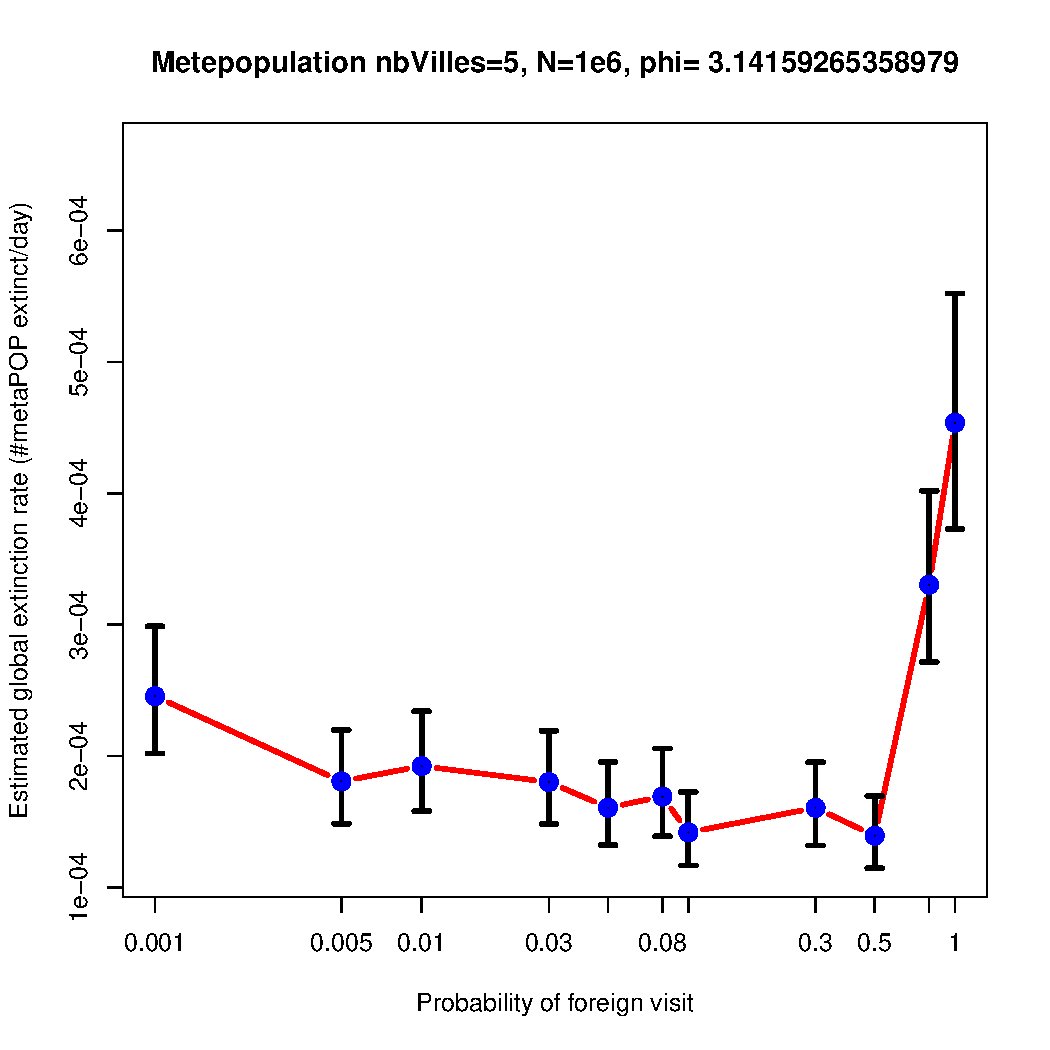
\includegraphics[scale=0.4]{plotprobVISITERVIl5N1e6PHIMAXpi_EXT}

\protect\caption{Correlation between the coupling rate and the mass extinction rate
in the metapopulation of five subpopulations. Here, the coupling rate
$\rho$ runs from 0 to 1. The level of asynchrony $\varphi_{max}$
is $\pi$ and the metapopulation size N=1e6.}
\end{figure}

\begin{itemize}
\item Running time : 8.884 hours
\item Analyse : One more factor that was pointed is coupling strength between
subpopulations. Here, the coupling rate or the dispersal rate $\rho$
can be considered as migration strength. The disease transmission
speed grows fast when coupling rate goes up in metapopulations, but
the global extinction rate is inverse. In this part, we permit coupling
rate change from weak to strong in a metapopualtion of five subpopulations
with the metapopulation size $N=10^{6}$. The dispersal rate $\rho$
is divided into three intervals. These are low, intermediate and high
coupling rate intervals. In each interval, we chose some coupling
rates that highlight the coupling strength among subpopulations in
a metapopulation. When the coupling rate is small from 0.0 to 0.005,
the mass extinction rate decreases very slowly. Because, in this case,
the subpopulations seem to be independent. They fluctuate independently.
They are easy to go extinct. We are also easy to find the mass extinction
in the metapopulation. However, this extinction rate is declined in
a sudden way when the coupling rate changes from 0.01 to 0.3. Lastly,
the extinction rate increases when the coupling rate is so robust
from 0.5 to 1.0. Based on this figure, the mass extinction rate in
a metapopulation is one inverse bell for the coupling rate. The medium
coupling rate (from 0.01 to 0.1) minimizes the mass extinction rate
in metapopulation. As in the case of the small and average coupling
rates, the coupling rate and the speed of migration among subpopulations
are directly proportional. The dispersal speed increases, thereby
the local recolonization speed rises, the duration of persistence
grows. However, this trend of global extinction rate with decreasing
coupling rate, is not right any more when the dispersal rate is strong.
The duration of persistence falls, because the metapopulation has
tendency to become one big population. In this case, the phase difference
or the recolonization among subpopulations are no longer significant.\end{itemize}

\end{document}
